\documentclass{resume} % Use the custom resume.cls style

\usepackage[left=0.75in,top=1in,right=0.75in,bottom=1in]{geometry} % Document margins
\usepackage{xcolor}
\usepackage{hyperref}
\hypersetup{
    colorlinks=true,
    linkcolor=blue,
    filecolor=magenta,      
    urlcolor=teal,
}
\usepackage{graphicx}
\newcommand{\tab}[1]{\hspace{.2667\textwidth}\rlap{#1}}
\newcommand{\itab}[1]{\hspace{0em}\rlap{#1}}
\newcommand{\spazio}{\begin{center} \par\noindent\rule{0.2\textwidth}{0.4pt} \end{center}}

\name{Emilio Berti} % Your name
\address{
    \centering
    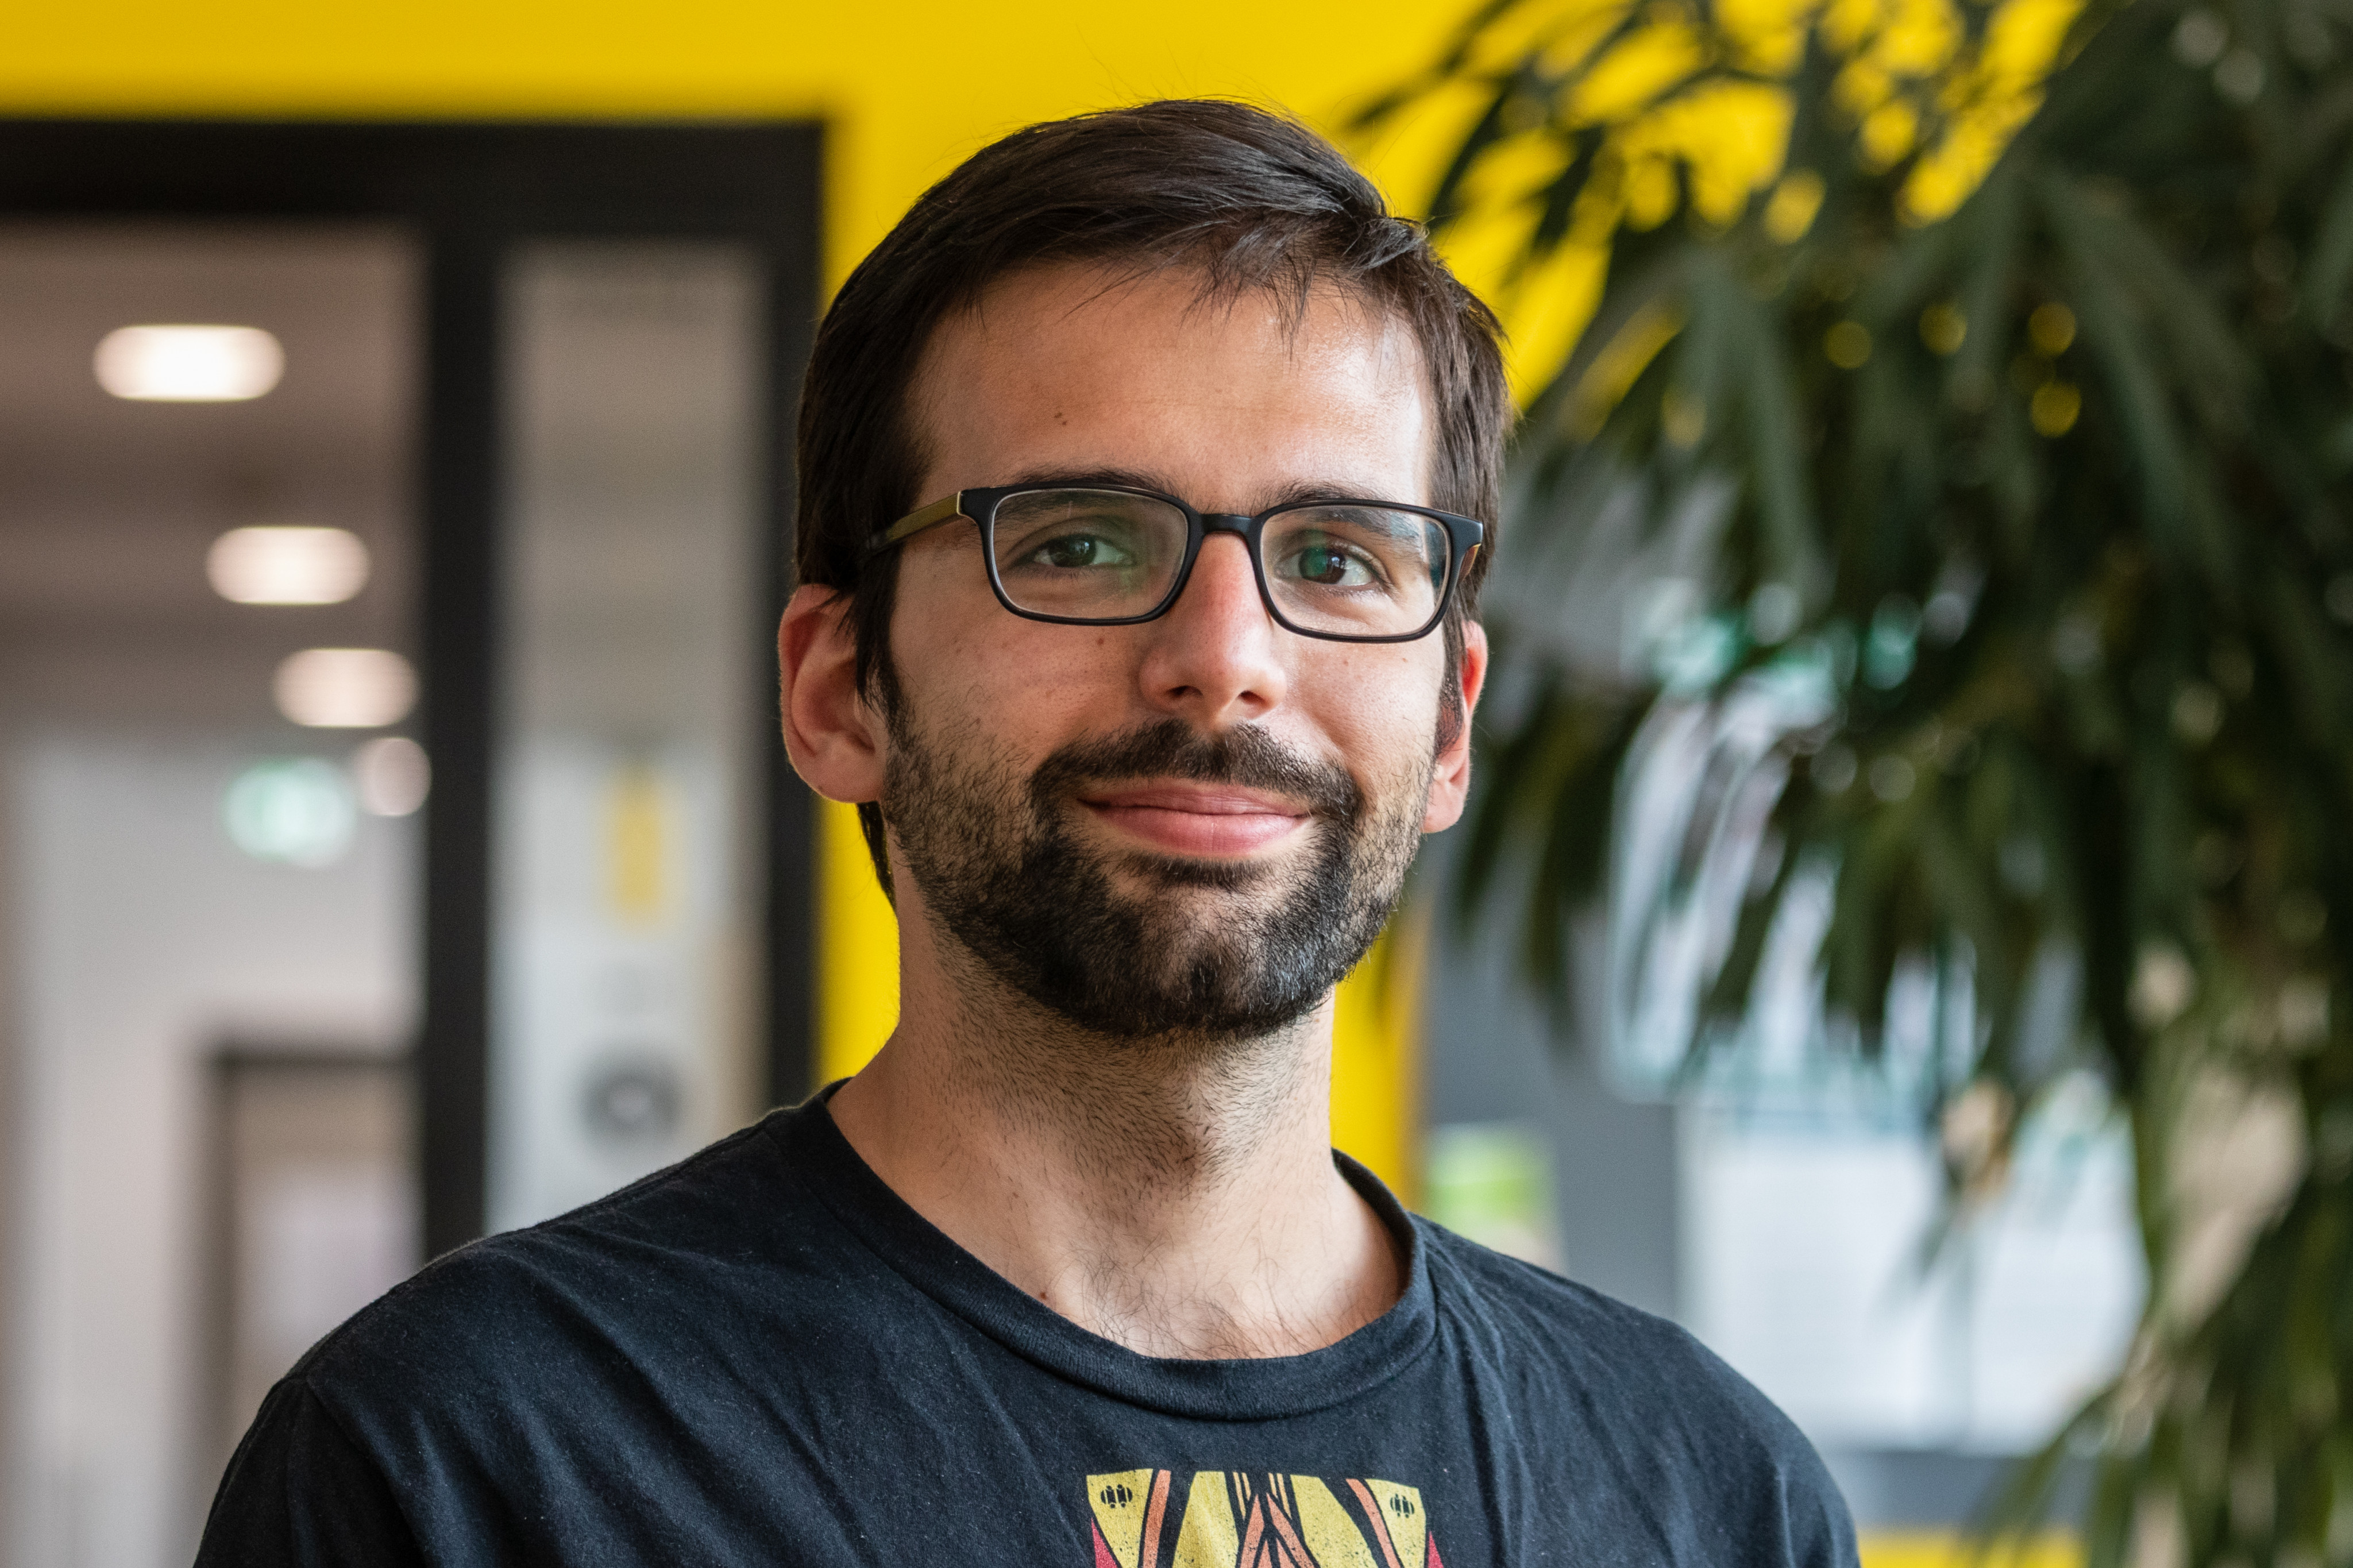
\includegraphics[width=0.30\textwidth]{Emilio.jpg}
}
\address{(+45) 266 54 662 \\ emilio.berti90@gmail.com}

\begin{document}

\begin{rSection}{Summary}
I am a theoretical ecologist with a passion for math and computing.
I have a strong quantitative background, with expertise in mathematical and statistical modelling of complex systems using big databases at large spatio-temporal scales.
I have worked in many different fields of biology, from molecular muscle physiology to macroecology and biogeography.
I am very open minded to other cultures and societies: I am Italian, my wife is Bulgarian, we met in Denmark, and we live in Germany.
I am an avid reader of ancient history and I love sumo.
\end{rSection}

\begin{rSection}{Professional Experience}
{\bf PostDoctoral researcher} \hfill {\em 01/10/2020 -- Present}\\
Theory in Biodiversity Science\\
German Centre for Integrative Biodiversity Research (iDiv)\\
Leipzig, Germany

In my current PostDoc position, I focus on theoretical ecology, community assembly, animal movement, and species' distribution models.

\spazio

{\bf Scientific consultant} \hfill {\em 01/05/2020 -- 31/07/2020}\\
Department of Bioscience\\
Aarhus University\\
Aarhus, Denmark

During these three months, I started developing a mechanistic model to assess areas of conservation priorities in Denmark using the national biodiversity database.

\spazio

{\bf Teaching assistant} \hfill {\em 01/02/2017 -- 30/04/2020}
\\Department of Biology\\
Aarhus University\\
Aarhus, Denmark

I taught one course every semester to fulfill the requirements of my PhD program. Teaching varied from lab support to lectures preparation and presentation.
\end{rSection}

\clearpage

\begin{rSection}{Education}
{\bf PhD} \hfill {\em 01/02/2017 -- 29/06/2020} 
\\ Section of Ecoinformatics and Biodiversity
\\ Department of Biology
\\ Aarhus University
\\ Aarhus, Denmark
\\ Title of dissertation: \textit{Megafauna extinctions, allometric scaling and biotic interactions: ecological effects and restoration opportunities through rewilding}.

{\bf Visiting PhD student} \hfill {\em 15/09/2018 -- 12/12/2018}
\\ Department of Ecology and Evolution
\\ University of Chicago
\\ Chicago, IL

{\bf MSc in Biology} \hfill {\em 01/09/2013 -- 31/04/2016}
\\ Department of Ecology and Evolution
\\ University of Florence
\\ Florence, Italy
\\ Title of dissertation: \textit{Analysis of the movement and aggressive interactions between two species of ants of the Genus Lasius (Hymenoptera: Formicidae) through mathematical models}.

{\bf BSc in Biology} \hfill {\em 01/09/2009 -- 31/09/2012}
\\ Department of Physiology
\\ University of Florence
\\ Florence, Italy
\\ Title of dissertation: \textit{The effects of myopalladin on the contraction mechanics of muscle fibers}.
\vskip3ex
\end{rSection}

\begin{rSection}{Skills}
I have acquired a very complementary set of skills through my career.
I have developed an outstanding mathematical and theoretical skill set through personal training and successfully applied it to investigate macroecological and biogeographical drivers of biodiversity.
I try to get the best from each experience; I have failed many times and will fail again, but this is also an opportunity to learn new things and incorporate them into my personal and professional growth.

\spazio

{\bf Languages}\\
Italian (native), English (fluent), Danish (beginner), German (beginner)\\
{\bf Programming}\\
R (expert), bash (expert), python (expert), C/C++ (advanced), javascript (mostly for Google Earth Engine, proficient), SQL (postgres flavour, advanced), GIS (expert)\\
{\bf Software} \\
Linux/GNU, QGIS, Anaconda, Jupyter Notebooks, \LaTeX, Git, GitHub\\
{\bf Methods} \\
Network analysis,
mathematical modeling,
Geographic Information Systems (GIS),
geoinformatics,
data science,
statistics,
ordination and classification,
optimization,
machine learning,
species distribution models (SDMs),
climate analyses,
environmental niche modeling,
high-performance clusters, 
automation.
\end{rSection}

\begin{rSection}{Scientific Publications}
% \vspace{4ex}\hfill{\em 2020}\\
\textbf{Berti, E.}, Rosenbaum, B., Brose, U., \& Vollrath, F. (2023). Energy landscapes direct the movement preferences of elephants. (Authorea; under review in Ecography). DOI: \url{https://doi.org/10.22541/au.168373276.62196439/v1}.\\
I was the leading author of this study, where I found that movement of elephants in Kenya is strongly determined by energetic costs of movement and availability of resources.

Dyer, A., Brose, U., \textbf{Berti, E.}, Rosenbaum, B., \& Hirt, M. (2023). Heat dissipation drives the hump-shaped scaling of animal dispersal speed with body mass. Plos Biology. DOI: \url{https://doi.org/10.1371/journal.pbio.3001820}.\\
I provided methodological advice and helped developing the mathematical model for this study, which shows that dispersal speed of animals is limited by their ability to dissipate heat produced during aerobic activity.

Terlau, J., Brose, U., Antunes, A. C., \textbf{Berti, E.}, Boy, T., Gauzens, B., ... \& Hirt, M. R. (2022). Integrating trait-based movement into mechanistic predictions of thermal performance.\\
I provided methodological advice and performed the thermal niche analysis for this study, which predicts the thermal limits of animals by integrating species traits with metabolic theory.

Gauzens, B., \textbf{Berti, E.}, Delmas, E., \& Brose, U. (2022). ATNr: Allometric trophic models in R. bioRxiv. (Under review at Methods in Ecology and Evolution as Gauzens, B., \dots, \& \textbf{Berti E.}).\\
I co-developed the code for this R package and supervised the integration of ATN models with R.

Bauer, B.*, \textbf{Berti, E.*}, ... \& Brose, U. (2022). Biotic filtering by species’ interactions constrains food-web variability across spatial and abiotic gradients. \textit{Ecology letters}. DOI: \href{https://doi.org/10.1111/ele.13995}{10.1111/ele.13995}. (\texttt{Shared first authorship}).\\
I shared first authorship of this paper, where we showed that species composition is determined by the interplay between environmental factors and species interactions using a global food-web database.

Grenié, M, \textbf{Berti, E.}, ... \& Marten, W. (2022). Harmonizing taxon names in biodiversity data: a review of tools, databases, and best practices. \textit{Methods in Ecology and Evolution}. DOI: \href{https://doi.org/10.1111/2041-210X.13802}{10.1111/2041-210X.13802}.\\
I co-developed the conceptual framework of this paper, where we identified current gaps in how ecological datasets are integrated for synthesis projects and suggested potential solutions. I also performed the analyses for the case study presented.

\textbf{Berti, E.}, Davoli, M., ... \& Vollrath, F. (2021). The r package enerscape: A general energy landscape framework for terrestrial movement ecology. \textit{Methods in Ecology and Evolution}. DOI: \href{https://doi.org/10.1111/2041-210X.13734}{10.1111/2041-210X.13734}.\\
I developed the R package and lead this study, where I integrate energy landscapes and GIS tools in order to provide macroecologists and conservation scientists with a null-model of animal movement based only on energetic costs of movement.\\
This paper received also a press release that drew attention of several media outlets, most notably the German national newspaper \textit{Die Welt} and the public radio broadcast \textit{Mitteldeutscher Rundfunk}, operating in the Federal States of Thuringia, Saxony and Saxony-Anhalt.

\textbf{Berti, E.}, Monsarrat, S., Munk, M., Jarvie, S. \& Svenning, J.C. (2020). Body size is a good proxy for vertebrate charisma. \textit{Biological Conservation}. DOI: \href{https://doi.org/10.1016/j.biocon.2020.108790}{10.1016/j.biocon.2020.108790}.\\
I lead and performed analyses of this study, where I show that humans are more positively attracted to animals, potentially biasing funding and conservation efforts towards protection of large animals, rather than species that are more critically endangered.

\textbf{Berti, E.} \& Svenning, J.C. (2020). Megafauna extinctions have reduced biotic connectivity worldwide. \textit{Global Ecology and Biogeography}. DOI: \href{https://doi.org/10.1111/geb.13182}{10.1111/geb.13182}.\\
I lead and performed analyses of this study, where I show how human-driven extinctions in the last 50,000 years have limited the ecosystem processes depending on animal dispersal.
\end{rSection}

\begin{rSection}{Peer review}
As of July 2022, I have reviewed 6 papers for: Ecography (2), Ecology Letters (2), GigaScience (1), and Scientia Agricola (1). You can find more at my \href{https://www.webofscience.com/wos/author/record/2190178}{WoS profile}.
\end{rSection}

\begin{rSection}{Conference talks}
\underline{Invited talk}: Bauer, B., \textbf{Berti, E.}, \dots, \& Brose, U. (2022). From regional to local scale: biotic interactions shape multilayer food-webs. \textit{SFE-GFO-EEF biannual meeting, Metz, France}.

\textbf{Berti, E.}, \& Svenning, J.C. (2022). State-space models show that functional replacements of extinct megafauna have distinct habitat preference in a European rewilding area. \textit{SFE-GFO-EEF biannual meeting, Metz, France}

Grenié, M., \textbf{Berti, E.}, Carvajal-Quintero, J., Winter, M., \& Sagouis (2021). Matching Species Names Across Biodiversity Databases: Sources, tools, pitfalls and best practices for taxonomic harmonization. \textit{TDWG annual meeting, online}

\textbf{Berti, E.} \& Svenning, J.C. (2019). Megalinkers extinction and the decrease of ecosystem connectivity. \textit{ESA annual meeting, Louisville, KY}

\textbf{Berti, E.}, Jarvie, S. W., \& Svenning, J.C. (2018). Rewiring food webs via trophic rewilding. \textit{BES annual meeting, Belfast, UK}
\end{rSection}

\begin{rSection}{Supervision and Mentoring}
I am informally co-supervising two PhD students at iDiv: Angelos Amyntas, whose work focuses on biodiversity-ecosystem functioning, and Ana Carolina Antunes, whose work focuses on the impacts of humans on $\alpha$-diversity using camera trap data. I am formally co-supervisor of the PhD candidate Jingyi Li, who is developing a novel mathematical approach for functional responses based on information theory. In addition to supervision, I also provide theoretical, computational, and statistical advice to several members of the TiBS working group at iDiv as well as individual mentoring for PhD students, advising especially on transferable skills and alternative career paths outside academia.
\end{rSection}

\begin{rSection}{Teaching \& Organized Workshops}
During my PhD, I taught one course every semester, as part of my salary was paid by Aarhus University on the basis of teaching.
I have thus a relatively long teaching experience for my career stage.
I also regularly organize lab workshops to teach reproducible research and open data principles.

\spazio

{\bf Teaching} \\
Introduction to scientific programming and tidyverse (2022) -- \href{https://emilio-berti.github.io/teaching/tidyverse.html#(1)}{slides}\\
Introduction to git and GitHub for a fool-proof programming (2022) -- \href{https://emilio-berti.github.io/idiv-git-introduction/}{course}\\
{\bf Teaching Assistant} \\
Theoretical Population Ecology (2023)
Meta-analyses for Biodiversity (2021)\\
Statistical and Geospatial Modelling (2019)\\
Behavioural Biology (2018, 2019)\\
Geographic Information System (2017)\\
{\bf Organized Workshops}\\
Cleaning online repository data for use in biogeography and macroecology (2019)\\
Running a species distribution model in R (2019)\\
A (very) gentle introduction to Linux (2019)
\end{rSection}

\begin{rSection}{Collaborations}
I have moved several times to pursue my career dreams and, being a friendly person, I established personal and professional ties with the people I met.
My network of current collaborators include:
\begin{itemize}
\setlength\itemsep{-0.5em}
    \item Prof. Jens-Christian Svenning, Aarhus University, Aarhus, Denmark.
    \item Prof. Ulrich Brose, Jena University, Jena, Germany.
    \item Prof. Daniel Reuman, Kansas University, Lawrence, KS, USA.
    \item Prof. Giacomo Santini, Universit\`{a} degli Studi di Firenze, Florence, Italy.
    \item Prof. Kai Yue, Fujian Normal University, Fuzhou, China.
    \item Prof. Neil Carter, University of Michigan, Ann Arbor, MI, USA.
    \item Ass. Prof. Susanne Vogel, Open University of the Netherlands, Heerlen, Netherlands.
    \item Prof. Fritz Vollrath, University of Oxford, Oxford, UK.
\end{itemize}
I also collaborate with Dr. Sophie Monsarrat, rewilding manager at the NGO Rewilding Europe (Nijmegen, Netherlands), and veterinary doctor Agnese Santi (Prato, Italy), with whom I am developing a new concept of ``wildness'' that can be applied to feral and semi-domesticated horses in Europe and that can lead to the identification of existing horse populations that promote biodiversity and ecosystem services.
\end{rSection}

\begin{rSection}{External Links}
\begin{minipage}{0.5\textwidth}
\begin{itemize}
    \item \href{https://scholar.google.com/citations?user=5KPh-oUAAAAJ&hl=en}{Google Scholar profile}
    \item \href{https://emilio-berti.github.io/}{Personal website}
    \item \href{https://orcid.org/0000-0001-9286-011X}{ORCiD}
\end{itemize}
\end{minipage}
\begin{minipage}{0.5\textwidth}
\begin{itemize}
    \item \href{https://www.linkedin.com/in/emilio-berti-55a348146}{LinkedIn}
    \item \href{https://github.com/emilio-berti}{GitHub}
    \item \href{https://publons.com/wos-op/researcher/4208953/emilio-berti/peer-review/}{Publons}
\end{itemize}
\end{minipage}
\end{rSection}

\end{document}
